% Chapter Template

\chapter{Control} % Main chapter title

\label{Chapter 2} % Change X to a consecutive number; for referencing this chapter elsewhere, use \ref{ChapterX}

\lhead{Chapter 2. \emph{Control}} % Change X to a consecutive number; this is for the header on each page - perhaps a shortened title

%
Once the simulation is fully implemented, the goal is to use it as a testbench for different ways of controlling the structure. The second part of the project will be fully consecrated on this part. A few tools have been implemented to test some of the algorithms that are used in such problems. 

\section{PID Control of the joints}

One of the problem to control accurately a joint is to adapt the command so that it can adapt to difficult situation. For instance, it is easier to walk in a swimmingpool than on the ground and this is why people recovering after an injury do aquatic training. For a joint, it can be easy to do a movement in the air, but the same movement is more difficult when touching the ground. One way to avoid this problem is to implement PID (Proportional Integral Derivative) controller. This kind of controller is used in a lot of different situation in the world of automation to control degrees of freedom. In or case, servomotors often integrate such loops to account for these changes of use. In the simulation, at each step, the command of each degree of freedom of the structure is calculated using such a PID controller. 


\begin{figure}[htbp]
    \centering
    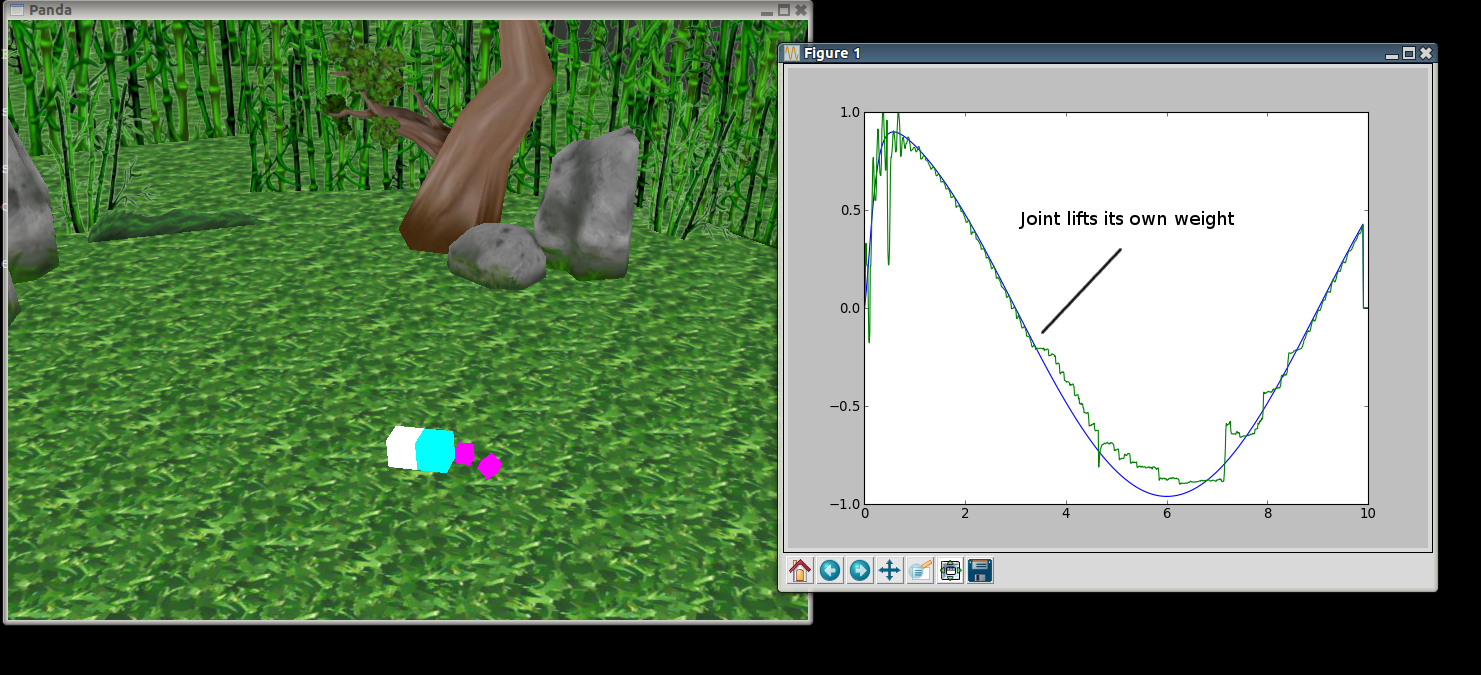
\includegraphics[scale=0.3]{Figures/servomotor.png}
    \rule{35em}{0.5pt}
    \caption[Answer of a joint to a sinusoid command]{Answer of the joint to a sinusoid command with PID Control}
    \label{fig:Snake}
\end{figure}


A few issues come from introducing PID in this problem. The stability is one of them. The PID loops need to be fast enough to be stable, which means that reducing the time between two steps of calculation on the physical world. The other problem is more a biological concern. The main goal of this project is to find solutions that are biologically inspired instead of using a classical automation approach. Therefore though the use of PID is necessary in many robotics applications, we will try to avoid using them in generating oscillations. 

\section{Central Pattern Generator}

Central Pattern Generators (CPGs) are neural networks, that can generate oscillation for the control of the muscles of or body. They are the consequence and the cause of the paradigm of periodic movement in the locomation of animals. Different models have been implemented to represent CPGs. We can represent them as a graph of coupled oscillator, where each node influence the behavior of its neighbours. 

## Equation of the chosen model

A modification of this model is possible to plug the measured value of the degrees of freedom. Thatway a direct control is possible without using the PID controllers. 

\section{Learning}

It is then possible to learn the parameters of the CPG to optimize the movement of the structure. Instead of having to find the value of the angles, the CPGs act as basis function for the angles, and thatway we reduce the space of research to a space with finite dimensions. 

